\section{Map}
\label{map}

Auf der Webseite habe ich die Google-Maps-API benutzt, um eine schnelle Überblick von allen Parks
zu schaffen. Die Google Maps Komponente wurde wie die \nameref{slideshow} Komponente über npm 
herunter geladen. Der Name der Komponente lautet \textit{google-map-react} und wurde von \textit{istarkov}
und \textit{itsmichaeldiego} erstellt. Ich habe auf der Seite zwei mal die Map benutzt. Der folgende 
Code ist die Map, wo alle Parks eingezeichnet sind.

\begin{lstlisting}
    const options = (maps) => {
        return {
            minZoom: 9,
            maxZoom: 20,
            disableDefaultUI: true,
            mapTypeControl: true,
            streetViewControl: true,
            styles: [{ featureType: 'poi', elementType: 'labels', stylers: [{ visibility: 'on' }] }],
        };
  };

    const defaultProps = {
        center: {
            lat: 47.2683,
            lng: 11.3933,
        },
        zoom: 11,
    };
    
    <GoogleMapReact
        options={options}
        bootstrapURLKeys={{ key: Keys }} //API-Key
        defaultCenter={defaultProps.center}
        defaultZoom={defaultProps.zoom}>
        {parks.map(park => (
            <Marker
            lat={park.latitude}
            lng={park.longitude}
            name={park.name}
            color="red"
            link={park.skateparkId}
            />  
        ))}
        {UserLangitude && <Marker
              lat={UserLangitude}
              lng={UserLongitude}
              name="Ihre Position"
              color = "blue"
            />}
      </GoogleMapReact>}
\end{lstlisting}

In den options, welche ich als Parameter der Komponente übergebe, wird der maximale und minimale Zoom 
definiert, der möglich sein soll. Außerdem werden viele Variablen mit dem Wert \textit{true} übergeben, 
welche verschiedene Google-Maps Eigenschaften wie zum Beispiel Street view aktivieren. Der API-Key \textbf{TODO API-KEY PHILLIP}
wird mittels \textit{useFetch} aus einer Textdatei ausgelesen, damit man diesem nicht im Quellcode zu 
finden ist. Innerhalb der park Variable, welche auch für die map verwendet wird, befinden sich alle 
Informationen aller Parks. In der Marker Komponente, wird dann der Breiten- und Längengrad als sowohl auch
der Parkname als Parameter übergeben. Es wird auch die Park ID als Parameter übergeben, um Innerhalb der 
Marker Komponente einen Link zu den Details des jeweiligen Parks zu ermöglichen. Drückt man also auf den Marker 
auf eines gewissen Parks, landet man auf dessen Details. Auf der Map wird ebenso ein Marker geladen, dem 
der Längengrad und Breitengrad des Benutzers übergeben wird, um eine bessere Orientierung der Umgebung 
zu ermöglichen.

\subsection{Marker}

Die Marker selbst sind eine einfache React-Komponente, welche auf die Position des angegeben Längen- und
Breitengrades platziert werden. 

\begin{figure}[H]
    \begin{center}
      \frame{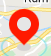
\includegraphics[width=0.1\textwidth]{Website/Marker.png}}
      \caption{Die Startseite}
    \end{center}
\end{figure}

Den Namen den man den Markern als Parameter übergibt, wird angezeigt, wenn sich die Maus über den 
Marker befindet. Übergibt man den Marker eine ParkID als link, kann dieser dazu benutzt werden die 
View zu einer \nameref{parkDetails}-View zu ändern. Übergibt man den Marker keinen Link Parameter
passiert beim Drücken des Markers nichts.